\documentclass[a4paper,11pt]{scrartcl}%scrbook %[...,twoside]

\usepackage[a4paper,left=3.5cm,right=2.5cm,bottom=3.5cm,top=3cm]{geometry}

\usepackage[ngerman]{babel}

% Caption Packet
\usepackage[margin=0pt,font=small,labelfont=bf]{caption}
% Gliederung einstellen
\setcounter{secnumdepth}{5}
%\setcounter{tocdepth}{5}
%\usepackage[Sonny]{fncychap}
%\ChTitleVar{\huge\rm}
\usepackage[pdftex]{graphicx,color}
\usepackage{amsmath,amssymb}
% Theorem-Umgebungen
\usepackage[amsmath,thmmarks]{ntheorem}
% Korrekte Darstellung der Umlaute
\usepackage[utf8]{inputenc}
\usepackage[T1]{fontenc}
\usepackage{lmodern}
\usepackage[onehalfspacing]{setspace}
% Algorithmen
 \usepackage[linesnumbered,ruled,vlined]{algorithm2e}
\usepackage{algorithmic}
%\renewcommand{\algorithmiccomment}[1]{\hfill \tiny//~#1\normalsize}
% Bibtex deutsch
\usepackage{bibgerm}
% URLs
\usepackage{url}
\usepackage{verbatim}

% Theorem-Optionen %
\theoremseparator{}
\theoremstyle{change}
\newtheorem{theorem}{Theorem}[section]
\newtheorem{satz}[theorem]{Satz}
\newtheorem{lemma}[theorem]{Lemma}
\newtheorem{korollar}[theorem]{Korollar}
\newtheorem{proposition}[theorem]{Proposition}
% Ohne Numerierung
\theoremstyle{nonumberplain}
\renewtheorem{theorem*}{Theorem}
\renewtheorem{satz*}{Satz}
\renewtheorem{lemma*}{Lemma}
\renewtheorem{korollar*}{Korollar}
\renewtheorem{proposition*}{Proposition}
% Definitionen mit \upshape
\theorembodyfont{\upshape}
\theoremstyle{change}
\newtheorem{definition}[theorem]{Definition}
\theoremstyle{nonumberplain}
\renewtheorem{definition*}{Definition}
% Kursive Schrift
\theoremheaderfont{\itshape}
\newtheorem{notation}{Notation}
\newtheorem{konvention}{Konvention}
\newtheorem{bezeichnung}{Bezeichnung}
\theoremsymbol{\ensuremath{\Box}}
\newtheorem{beweis}{Beweis}
\theoremsymbol{}
\theoremstyle{change}
\theoremheaderfont{\bfseries}
\newtheorem{bemerkung}[theorem]{Bemerkung}
\newtheorem{beobachtung}[theorem]{Beobachtung}
\newtheorem{beispiel}[theorem]{Beispiel}
\newtheorem{problem}{Problem}
\theoremstyle{nonumberplain}
\renewtheorem{bemerkung*}{Bemerkung}
\renewtheorem{beispiel*}{Beispiel}
\renewtheorem{problem*}{Problem}
%
%% Algorithmen anpassen %
%\renewcommand{\algorithmicrequire}{\textit{Eingabe:}}
%\renewcommand{\algorithmicensure}{\textit{Ausgabe:}}
%\floatname{algorithm}{Algorithmus}
%\renewcommand{\listalgorithmname}{Algorithmenverzeichnis}
%\renewcommand{\algorithmiccomment}[1]{\color{grau}{// #1}}
%
% Floating-Umgebungen anpassen %
\renewcommand{\topfraction}{0.9}
\renewcommand{\bottomfraction}{0.8}
% Abkuerzungen richtig formatieren %
\usepackage{xspace}
\newcommand{\vgl}{vgl.\@\xspace} 
\newcommand{\zB}{z.\nolinebreak[4]\hspace{0.125em}\nolinebreak[4]B.\@\xspace}
\newcommand{\bzw}{bzw.\@\xspace}
\newcommand{\dahe}{d.\nolinebreak[4]\hspace{0.125em}h.\nolinebreak[4]\@\xspace}
\newcommand{\etc}{etc.\@\xspace}
\newcommand{\evtl}{evtl.\@\xspace}
\newcommand{\ggf}{ggf.\@\xspace}
\newcommand{\bzgl}{bzgl.\@\xspace}
\newcommand{\so}{s.\nolinebreak[4]\hspace{0.125em}\nolinebreak[4]o.\@\xspace}
\newcommand{\iA}{i.\nolinebreak[4]\hspace{0.125em}\nolinebreak[4]A.\@\xspace}
\newcommand{\sa}{s.\nolinebreak[4]\hspace{0.125em}\nolinebreak[4]a.\@\xspace}
\newcommand{\su}{s.\nolinebreak[4]\hspace{0.125em}\nolinebreak[4]u.\@\xspace}
\newcommand{\ua}{u.\nolinebreak[4]\hspace{0.125em}\nolinebreak[4]a.\@\xspace}
\newcommand{\og}{o.\nolinebreak[4]\hspace{0.125em}\nolinebreak[4]g.\@\xspace}
\newcommand{\oBdA}{o.\nolinebreak[4]\hspace{0.125em}\nolinebreak[4]B.\nolinebreak[4]\hspace{0.125em}d.\nolinebreak[4]\hspace{0.125em}A.\@\xspace}
\newcommand{\OBdA}{O.\nolinebreak[4]\hspace{0.125em}\nolinebreak[4]B.\nolinebreak[4]\hspace{0.125em}d.\nolinebreak[4]\hspace{0.125em}A.\@\xspace}

% Leere Seite ohne Seitennummer, naechste Seite rechts
\newcommand{\blankpage}{
 \clearpage{\pagestyle{empty}\cleardoublepage}
}
\bibliographystyle{unsrt}
\usepackage{hyperref}
% Keine einzelnen Zeilen beim Anfang eines Abschnitts (Schusterjungen)
\clubpenalty = 10000
% Keine einzelnen Zeilen am Ende eines Abschnitts (Hurenkinder)
\widowpenalty = 10000 \displaywidowpenalty = 10000
% EOF
\titlehead{
	\begin{minipage}{7.2cm}
		\vspace{-6mm}
		\hspace{-4mm}
	
\includegraphics[scale=0.5]{./logo}
	\end{minipage}
	\begin{minipage}{7.6cm}
		\begin{flushright}
			Fakultät für Informatik\\
			Lehrstuhl für Algorithm Engineering (LS11)\\
			http://ls11-www.cs.tu-dortmund.de\\
		\end{flushright}
  \end{minipage}
  \\
	\centerline{\hrulefill}
}%end of titlehead


\title{\vspace{2,5cm}Textkompression mithilfe einer Variante von LZ78}
\subtitle{Bachelorarbeit}
\author{Florian Kleine\\Matrikelnummer: 157020}
\publishers{\parbox[b][12cm]{\textwidth}{Betreuer:\\ Prof. Dr. Johannes Fischer\\
Dominik Köppl}}
\date{\today}



\begin{document}
\maketitle
\thispagestyle{empty}
\newpage
\tableofcontents
\newpage
\newpage

\section{Einleitung}
Die Datenkompression spielt in der Informatik eine große Rolle. Zwar sind die Datenträger im Vergleich zu früher um ein Vielfaches größer und vor allem günstiger geworden, stoßen bei den heute anfallenden riesigen Datenmengen aber immer noch an ihre Grenzen. Deshalb ist es sinnvoll die Daten mit geschickten Verfahren so zu komprimieren, dass sie später verlustfrei in den Ursprungszustand zurückübersetzt werden können.
In dieser Arbeit soll es darum gehen, Texte mithilfe einer Variante des Lempel-Ziv78-Verfahrens in Faktoren zu zerlegen, zu kodieren und so verlustfrei zu komprimieren. Dieses Verfahren stützt sich auf der Eliminierung von Redundanzen, indem Teile des Textes durch Verweise auf vorher auftretende gleiche Teile ersetzt werden. Solche Verweise benötigen weniger Speicher als der Text, was so zu einer Kompression des kompletten Textes führt.
Das aus dieser Arbeit entstehende Verfahren wird anschließend mit bereits vorhandenen Kompressionsverfahren (z.B. gzip und 7zip) verglichen.\\\\

\subsection{Anekdote}
Um die Bedeutung von Datenkompression zu verdeutlichen und zu zeigen, wie lange man sich über dieses Thema schon Gedanken macht, hier eine kleinen Anekdote:\\
Ende des 18. Jahrhunderts benötigte die britische Marine eine schnelle Kommunikation zwischen London und dem Marinestützpunkt an der Küste. Dies wurde durch eine Kette von Hütten auf Hügeln in etwa 5 Meilen Entfernung umgesetzt. Diese Hütten(sog. \textit{Klappentelegraphen}\ref{fig:braille}) hatten 6 Klappen auf dem Dach, die entweder geschlossen oder geöffnet waren. Durch diese 64 möglichen Kombinationen von offenen und geschlossenen Klappen konnte man Buchstanden des Braille-Alphabets\ref{fig:braille} darstellen. Da das Alphabet weniger als 64 Buchstaben hat, gab es freie Kombinationen von Klappenstellungen. Diese freien Kombinationen wurden dazu benutzt die Kommunikation zu beschleunigen. Oft benutzen Wörtern wie 'for' oder 'the' wurden freie Kombinationen zugewiesen. Anderen Worten wie 'father' oder 'mother' wurde die freie Kombination 'dot5' und die Kombination für 'f' bzw. 'm' zugewiesen. So erreichte man eine Kompression von 20\% bei englischen Texten.\cite[S.1-4]{bellTextCompression} \\
Dieses Problem hat sich bis heute nicht geändert. Wie verringern wir die Datenmenge möglichst stark und beschleunigen somit die Übertragung, ohne Informationen zu verlieren?
	\begin{figure}[h]
	
		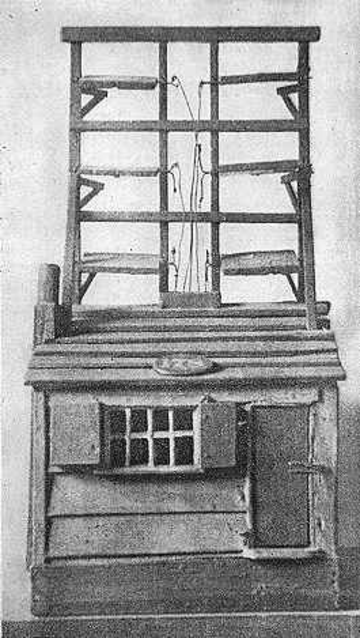
\includegraphics[scale=0.25]{./pics/shuttercabin}\cite{klappentelegraph}
		\hspace{25pt}
	 	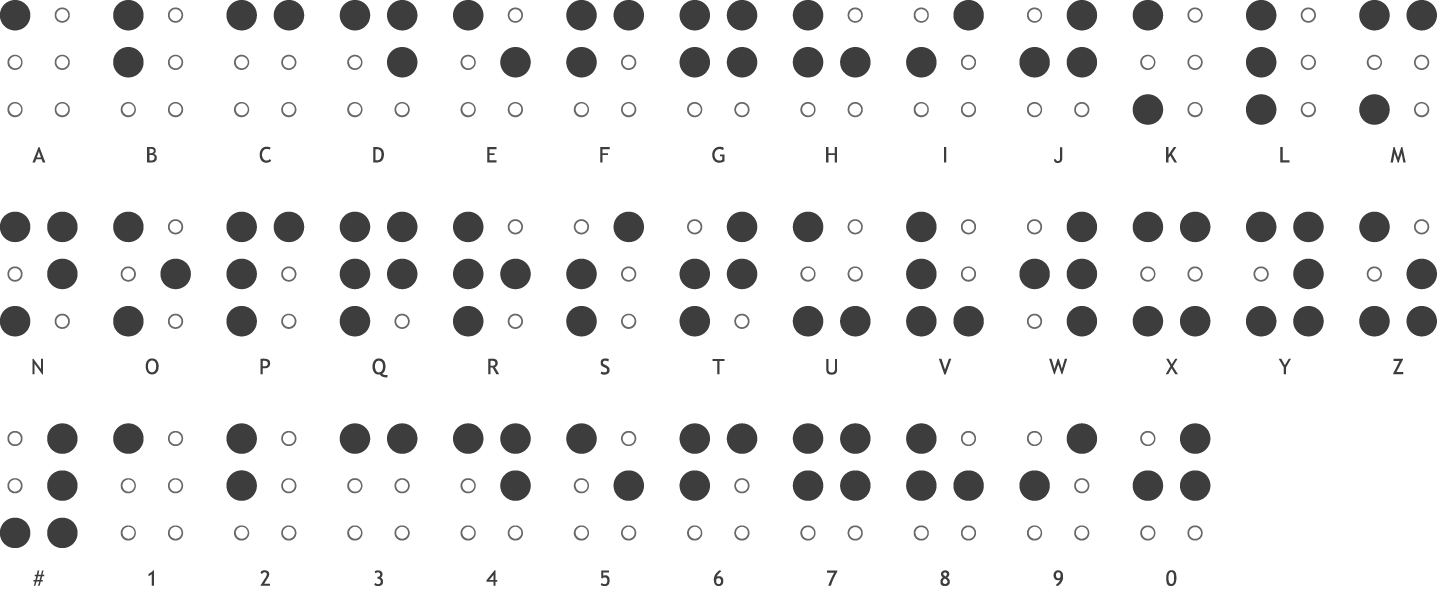
\includegraphics[scale=0.17]{./pics/braille}\cite{braille}
	 	\caption{Links sieht man einen Klappentelegraphen. Rechts das englische Braille-Aphabet. }
	  	\label{fig:braille}
	\end{figure}
\newpage
\section{Theoretische Grundlagen}

Im Folgenden werden Datenstrukturen und Operationen eingeführt, die wir in dieser Arbeit benötigen werden.

\subsection{Operationen auf Strings}

Sei das Alphabet $\Sigma$ definiert als eine Menge von Zeichen, dann bezeichnet $\Sigma^{*}$ die Menge aller Worte, die aus dem Alphabet gebildet werden können. Jedes dieser Worte bezeichnet man als String.
	Sei $s$ ein String mit der Länge $n$.
	
	\begin{definition}[Länge]
		Sei $|s|$ die Länge des String $s$, das heißt die Anzahl von Zeichen in $s$.
	\end{definition}
	
	\begin{definition}[Leerstring]
		Sei $\varepsilon \in \Sigma$* der leere String. Es gilt $|\varepsilon|$ = 0.
	\end{definition}
	
	\begin{definition}[Symbolzugriff]
		Für $x \in \mathbb{N}$ und $x \leq n$ sei $s[x]$ das $x$-te Zeichen aus $s$.
	\end{definition}
	
	\begin{definition}[Teilstring]
		Für $x,y \in \mathbb{N}$ und $1 \leq x < y \leq n$ sei $s[x,y]$ die Zeichenfolge vom $x$-ten bis zum $y$-ten Zeichen aus $s$. $s$[x] und $s$[y] einschließlich.
	\end{definition}
	
	\begin{definition}[Suffix]
		 Für $x \in \mathbb{N}$ und $x \leq n$ sei $s[x..]$ das $x$-te Suffix von $s$. Also gilt $s[x..] = s[x,n]$.
	\end{definition}
	
\subsection{Suffix-Tree}

\begin{definition}[Suffix-Tree]
		Ein Suffix-Tree eines Strings $s$ ist ein Baum mit $n$ Blättern. Alle inneren Knoten erfüllen folgende Bedingungen:
		\begin{itemize}
			\item Jeder Knoten hat mindestens 2 Kinder.
			\item Jede Kante ist mit einem nicht-leeren Teilstring von $s$ markiert.
			\item Die Markierung ausgehender Kanten eines Knotens beginnen nicht mit dem gleichen Zeichen.
			\item Die Konkatenation von allen Zeichen auf dem Pfad von der Wurzel zum Blatt $i$ ist das $i$-te Suffix $s[i..]$ von $s$.
		\end{itemize}
		\begin{beispiel}[Suffix-Tree]
			$s$ = \texttt{ananas\$}
			\begin{figure}[h]
				\centering
				  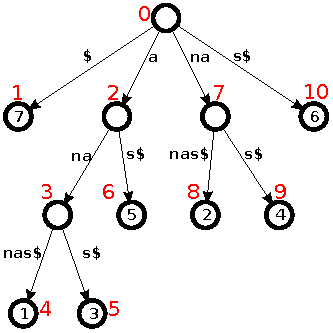
\includegraphics[scale=0.8]{./pics/ananas_suffixTree_inorder}
				  \cite{suffixtreeurl}
				  \caption{Diese Abbildung zeigt den Suffix-Tree zu $s$ = \texttt{ananas\$}. Die Blätter sind hierbei nummeriert. Der String auf dem Pfad von der Wurzel zum Blatt $i$ repräsentiert das Suffix $s[i..]$. Die roten Zahlen an den Knoten sind durch eine Pre-Order-Nummerierung entstanden und sind die IDs der Knoten. }
				  \label{fig:suffixTree}
			\end{figure}
		\end{beispiel}
		
	\end{definition}
	
\subsection{Min-Heap}

Ein \textbf{(binärer) Heap} ist ein Binärbaum, dessen Knoten je ein Element einer Menge $X$ enthalten. Jeder Knoten erfüllt bezüglich einer totalen Ordnung $(X,\preceq)$ die \textit{Heap-Eigenschaft}. Diese Eigenschaft ist wie folgt definiert:

\begin{definition} [Heap-Eigenschaft]
	\textbf{Gegeben:} Eine Menge $X$ und eine Relation $\preceq$.\\
	Sei $x_{l}$ der linke und $x_{r}$ der rechte Kindknoten von $x$, so gilt:\\
	\begin{center}{$x_{l} \preceq x$ und $x_{r} \preceq x$}\end{center}
	 
\end{definition}

Ein \textit{Min-Heap} ist ein Heap, dessen Elemente die Relation $\geq$ erfüllen. Das heißt jeder Kindknoten enthält ein Element, das mindestens so groß ist wie das seines Elternknotens. Abbildung \ref{fig:min_heap_example} zeigt beispielhaft einen \textit{Min-Heap} $(\mathbb{N}, \geq )$.

\begin{figure}[h]
	    \centering
		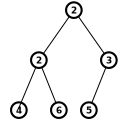
\includegraphics[scale=0.9]{./pics/min_heap_example}
		 \caption{Beispiel eines \textit{Min-Heaps} $(\mathbb{N}, \geq )$.}
		 \label{fig:min_heap_example}
\end{figure}
\newpage

Eine effiziente Darstellung eines \textit{Heaps} ist ein Array $H$, was folgende Eigenschaften erfüllt:

\begin{itemize}
	\item Die erste Stelle von $H$ ist die Wurzel des Baums. \label{heap_array_prop_1}
	\item Der linke Kindknoten des $i-ten$ Knotens steht an der Stelle $2i$.
	\item Der rechte Kindknoten des $i-ten$ Knotens steht an der Stelle $2i + 1$.
	\item Der Vaterknoten des $i-ten$ Knotens steht an der Stelle $\lfloor\frac{i}{2}\rfloor$. ($i>1$)
\end{itemize}
	
In Abbildung \ref{fig:array_heap} sehen wir die Array-Darstellung des Baums aus Abbildung \ref{fig:min_heap_example}.

\begin{figure}[h]
	\centering
	
		\begin{tabular}[h]{|l|c|c|c|c|c|c|}\hline
			$i$ & 1 & 2 & 3 & 4 & 5 & 6\\ \hline
		   H[$i$] & 2 & 2 & 3 & 4 & 6 & 5\\ \hline
		   
		\end{tabular} 
		\caption{Array-Darstellung des Baums aus Abbildung \ref{fig:min_heap_example}.}
		\label{fig:array_heap}
\end{figure}

Ein Zugriff auf das kleinste Element des \textit{Min-Heaps} ist in $O(1)$ Zeit möglich, da das kleinste Element des Heaps immer an der ersten Stelle liegt.
Fügen wir ein neues Element in den Heap ein oder Löschen ein Element, so muss die \textit{Heap-Eigenschaft} weiterhin gelten. Daher benötigen Einfüge- und Löschoperationen $O(\log n)$ Zeit, wenn der Heap $n$ Elemente enthält. \cite[S.115ff]{introductionToAlgorithms}

	
\section{Idee der LZ78 Variante}

Um die Grundidee des Verfahrens, das wir in dieser Arbeit entwickeln, zu erläutern, betrachten wir im Folgenden zunächst LZ78.

\subsection{LZ78}\label{lz78_sec}

LZ78 wurde 1978 von Jacob Ziv und Abraham Lempel erfunden und ist ein Verfahren zur Textkompression. Es benutzt dabei ein \textit{adaptives Wörterbuch}, das heißt für jeden Eingabetext wird ein anderes Wörterbuch erzeugt. LZ78 unterteilt den Eingabetext in Faktoren. Dabei ist jeder Faktor der längste, gleiche Substring im bisher gelesenen Eingabetext plus das nächste Zeichen. Ein Faktor wird dabei als Tupel $(x,c)$ dargestellt, wobei $x$ der Index des Prefix ist und $c$ das zusätzliche Zeichen. Eine Einschränkung, wie weit der referenzierte Teilstring zurückliegen darf, gibt es hierbei nicht. Wenn $p$ Faktoren erstellt wurden, lässt sich der Index mit $\lceil\log p\rceil$ Bits darstellen. In der Praxis kann dieses Wörterbuch nicht unendlich groß werden. Daher löscht man dieses Wörterbuch, falls kein Speicher mehr verfügbar ist, und arbeitet mit einem leeren Wörterbuch und dem restlichen Eingabetext weiter.\\
Eine effiziente Datenstruktur, um die Faktoren darzustellen, ist ein Trie bzw. hier der sog. LZ78-Trie. Jeder Knoten des LZ78-Tries enthält den Index des Faktors, den er repräsentiert. Hierbei ist $s_{Pfad} = s_{Faktor}$, wenn $s_{Pfad}$ der String auf dem Pfad von der Wurzel bis zum Knoten ist und $s_{Faktor}$ der durch den Faktor dargestellte Teilstring des Eingabetextes.\cite[S.225]{bellTextCompression}\\
Dieses Verfahren wird in Abbildung \ref{fig:lz78} nun am Beispiel von $T = \texttt{ananas\$}$ verdeutlicht:

 	
	\begin{figure}[h]
	\begin{tabular}[t]{cc}
		\begin{tabular}[b]{l c c c c c}\hline
			& 1 & 2 & 3 & 4 & 5 \\ \hline
		   Textteil & \texttt{a} & \texttt{n} & \texttt{an} & \texttt{as} & \texttt{\$}\\ \hline
		   Faktorzerlegung & (-,\texttt{a}) & (-,\texttt{n}) & (1,\texttt{n}) & (1,\texttt{s}) &  (-,\texttt{\$})\\ \hline
		\end{tabular} & 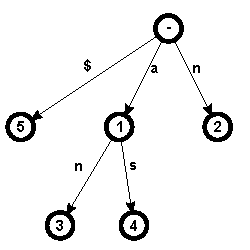
\includegraphics{./pics/ananas_LZ78Tree}
	\end{tabular}
	\caption{Links sieht man die Faktorisierung nach LZ78 und rechts den entsprechenden LZ78-Tree. Der $i$-te Faktor $(x,s)$ wird zu einem neuen Knoten $i$ mit $x$ als Elternknoten und die Kante $(x,i)$ wird mit $s$ beschriftet.}
	\label{fig:lz78}
	\end{figure}

	
	

\subsection{LZ78 Variante}\label{LZ78 Variante}

In dieser Arbeit wollen wir eine Variante (im Folgenden LZ78V genannt) zu LZ78 aus Kapitel \ref{lz78_sec} entwickeln. LZ78V unterteilt den Eingabetext auch in Faktoren. Jedoch kann ein Faktor mehr als nur das nächste Zeichen an den referenzierten Teilstring anhängen. Die Information, welche Zeichen dies sind, bezieht LZ78V aus dem Suffix-Tree. Bei unserem Beispieltext $T = \texttt{ananas\$}$ folgt nach einen \texttt{'n'} immer ein \texttt{'a'}. Dies spiegelt sich im Suffix-Tree aus Abbildung \ref{fig:suffixTree} durch die Kante (0,7), die mit \texttt{'na'} beschriftet ist, wider. Mit LZ78V können wir nun beim ersten Lesen von \texttt{'n'} den Faktor (0, \texttt{'na'}) erstellen.
 Es ergibt sich die Faktorisierung aus Abbildung \ref{fig:lz78v}. \\\newpage
	\begin{figure}[h]
	\begin{tabular}[t]{c c c}
		\begin{tabular}[b]{l c c c}\hline
			& 1 & 2 & 3  \\ \hline
  		Textteil & \texttt{a} & \texttt{na} & \texttt{nas\$} \\ \hline
  		Faktorzerlegung & (-,\texttt{a}) & (-,\texttt{na}) & (2,\texttt{s\$}) \\ \hline
		\end{tabular} & \hspace{2cm} & 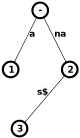
\includegraphics{./pics/ananas_LZ78VTree}\\\\
	\end{tabular}
	\caption{Links sieht man die Faktorisierung nach LZ78V und rechts den entsprechenden LZ78V-Tree. Der $i$-te Faktor $(x,s)$ wird zu einem neuen Knoten $i$ mit $x$ als Elternknoten und die Kante $(x,i)$ wird mit $s$ beschriftet. Im Gegensatz zum LZ78-Tree kann $s$ aber mehr als ein Zeichen beinhalten.}
	\label{fig:lz78v}
	\end{figure}
	
	Den LZ78V-Tree können wir mit einem zweidimensionalen Array $A$ repräsentieren. So wäre $A[i][1] = x$ und $A[i][2] = s$ der $i$-te Faktor $(x,s)$ in der Array-Darstellung. Im Beispiel $T$ = \texttt{ananas\$} ergibt sich:\\\\
	\begin{tabular}{l c c c}
						\hline
							& 1 & 2 & 3 \\\hline
						$A[1]$ & - & - & 2 \\\hline
						$A[2]$	& \texttt{a} & \texttt{na} & \texttt{s\$}\\\hline
						
			
	\end{tabular}\\
	
LZ78V baut also wie LZ78 einen Tree auf. Vergleichen wir beide Trees aus unserem Beispiel, fällt auf, dass der LZ78V-Tree zwei Knoten weniger hat. Das heißt wir müssen weniger Informationen abgespeichert. Eine Kodierung des LZ78V-Trees entwickeln wir in einem späteren Abschnitt.\\
Gehen wir jedoch strikt nach dem oben beschriebenen Verfahren vor, so kann es auch zu einer schlechteren Faktorisierung als bei LZ78 kommen. Schlecht definieren wir hier über die Gesamtanzahl der Zeichen in der Faktorisierung. Je mehr Zeichen, desto schlechter ist die Faktorisierung. Betrachten wir beispielsweise den Text $T = \texttt{kananas\$}$. Lesen wir nun das \texttt{'k'} erstellt LZ78V direkt den Faktor $(-, \texttt{kananas\$})$ mit 8 Zeichen. Dies entsteht dadurch, dass sobald wir ein \texttt{'k'} lesen, LZ78V den kompletten String der Kante (0,7) des Suffix-Trees aus Abbildung \ref{fig:kananas} zu einem Faktor hinzufügt. Da \texttt{'k'} ein einzigartiges Zeichen in $T$ ist, enthält der Faktor des gesamten Text $T$. In dieser Arbeit soll hierfür eine Lösung gefunden werden. Es wäre zum Beispiel denkbar, $(x,s)$ mit $x \in \{1...z\} \cup \{-\}$ und $s \in \Sigma^{+}$ nur in die Faktorisierung aufzunehmen, wenn der entsprechende Knoten im Suffix-Tree kein Blatt ist. Ansonsten nehmen wir nur das erste Zeichen von $s$.\\ Am Beispiel von $T = \texttt{kananas\$}$ ergibt somit folgeneder LZ78V-Tree in der Array-Darstellung:\\

\begin{tabular}{l c c c c c}
						\hline
							& 1 & 2 & 3 & 4 & 5\\\hline
						$A[1]$ & - & - & - & 3 & -\\\hline
						$A[2]$	& \texttt{k} & \texttt{a} & \texttt{na} & \texttt{s} & \texttt{\$}\\\hline
						
			
\end{tabular}\\




\begin{figure}[h]
	    \centering
		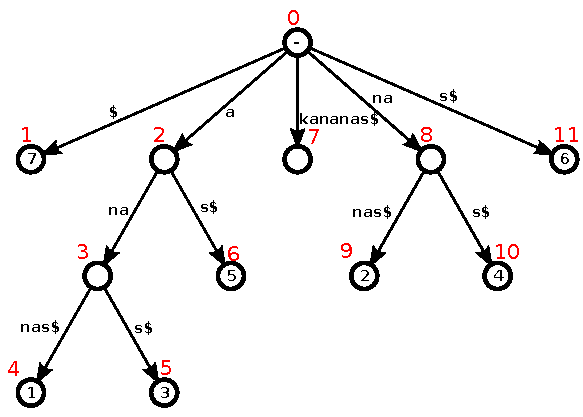
\includegraphics[scale=0.75]{./pics/kananas_suffixTree_inorder}
		 \caption{Diese Abbildung zeigt den Suffix-Tree zu $s$ = \texttt{kananas\$}. Die Blätter sind hierbei nummeriert. Der String auf dem Pfad von der Wurzel zum Blatt $i$ repräsentiert das Suffix $s[i..]$. Die roten Zahlen an den Knoten sind durch eine Pre-Order-Nummerierung entstanden und sind die IDs der Knoten.}
		 \label{fig:kananas}
\end{figure}

Diese Faktorisierung hat insgesamt 6 Zeichen, ist also besser als die Faktorisierung nach dem strikten Verfahren.

\section{Textkompression mit LZ78V}

\subsection{Faktorisierung}

In diesem Kapitel entwickeln wir einen Algorithmus und die dazu notwendigen Datenstrukturen, basierend auf der Grundidee aus Abschnitt \ref{LZ78 Variante}. 
Desweiteren definieren wir einen \textit{Kodierer}, der die Faktorisierung kodiert und wir sie so effizient abspeichern können.
Abschließend stellen wir einen \textit{Dekodierer} vor, der aus einer Kodierung wieder eine Faktorisierung aufbaut.

\begin{algorithm}[t]
	\SetAlgoLined
	\KwData{Eingabetext $T$}
	\KwResult{Vector mit IDs, Repräsentation der Faktoren}
	
	konstruiere Suffix-Tree aus $T$\;
	erstelle Bit-Vektor $used$ und Int-Vektor $factors$\;
	\While{Textende nicht erreicht} {
		suche anhand des aktuellen Zeichens den nächsten Knoten im Suffix-Tree\;\label{line:child}
		\If{$used$[aktueller Knoten]}{ \label{line:used}
			setze Textposition entsprechend der Zeichen an der Kante weiter\;
			continue\;
		}
		\If{aktueller Knoten ist ein Blatt}{ \label{line:onlyFirstSym}
			setze Textposition um 1 weiter\;
		} \Else {
			setze Textposition entsprechend der Zeichen an der Kante weiter\; \label{line:textpos}
		}
		füge die ID des aktuellen Knotens an $factors$ an\;
		markiere aktuellen Knoten in $used$ als benutzt\;
	}
	
	\caption{LZ78V Faktorisierung mit Vektoren}
	\label{algo:factVec}
\end{algorithm}
\newpage
\subsubsection{SDSL-lite}
SDSL-lite ist eine C++11 Bibliothek, die speichereffiziente Datenstrukturen zur Verfügung stellt. Die benutzen Datenstrukturen dieser Bibliothek werden im Nachfolgenden an den passenden Stellen eingeführt.\cite{sdsl}

\subsubsection{Suffix-Tree Konstruktion}

Um aus dem Eingabetext einen Suffix-Tree zu konstruieren verwenden wir die Bibliothek SDSL-lite. Hiermit können wir einen sog. \textit{Compressed Suffix Tree} (CST) erzeugen. Dieser hat zur Laufzeit einen Speicherbedarf von 3$n$ + o($n$) + $\arrowvert$CSA$\arrowvert$ + $\arrowvert$LCP$\arrowvert$ Bits .\cite{sdsl} Jeder Knoten besitzt eine ID $i$, die wir durch eine Anfrage an den Baum in konstanter Zeit erhalten.
Sei $x$ die Anzahl von Knoten im Suffix-Tree, dann gilt:
\begin{center}
	$i \in [0..x]$
\end{center}

\subsubsection{Vektoren}

Der Algorithmus benutzt drei Vektoren. Diese erstellen wir wieder mithilfe von SDSL-lite.

\paragraph{Bit-Vektor used}

Der Bit-Vektor $used$ besteht aus $x$ Bits, die mit 0 initialisiert werden. Dieser Vektor gibt an, ob ein Knoten mit der ID $i$ schon als Faktor benutzt wird.
Ist dies der Fall, so ist $used[i]=1$. Dieser Vektor benötigt $64*\lceil\dfrac{n}{64}+1\rceil$ Bits.\cite{sdsl}

\paragraph{Int-Vektor factors}

Der Int-Vektor $factors$ ist zu Beginn leer. Wir füllen ihn im Laufe der Faktorisierung mit IDs von Knoten aus dem Suffix-Tree.  

\subsubsection{Abbruchbedingung}

Der Algorithmus bricht dass ab wenn wir das Ende des Eingabetextes erreicht haben. Dies ist der Zeitpunkt, an dem die Faktorisierung abgeschlossen ist.

\subsubsection{Faktoren erstellen}

Der Startknoten jedes neuen Suchdurchlaufs ist die Wurzel des Suffix-Trees.
In Zeile \ref{line:child} des Algorithmus \ref{algo:factVec}  suchen wir anhand des aktuellen Zeichens aus dem Text den nächsten Knoten $k$ im Suffix-Tree. Diese Methode wird von SDSL-lite bereitgestellt und benötigt $O((t_{SA}+t_{SA^{-1}}) * \log \sigma + t_{LCP})$ Zeit. Hierzu sehen wir in einem späteren Abschnitt noch eine schnellere Alternative. In Zeile \ref{line:used} testen wir, ob $k$ schon als Faktor benutzt wird. Das bedeutet, wir haben den String  auf dem Pfad bis $k$ bereits durch einen Faktor dargestellt und können diesen nun referenzieren. Falls dies der Fall ist, setzen wir die Textposition um so viele Zeichen weiter, wie an der Kante zu $k$ stehen und suchen nach dem nächsten Knoten. Sobald wir einen Knoten $k$ gefunden haben, der noch nicht als Faktor benutzt wird, also für den $used[k]$ = 0 gilt, testen wir in Zeile \ref{line:onlyFirstSym}, ob der aktuelle Knoten ein Blatt ist. Falls ja, erhöhen wir die Textposition nur um 1, da nur das erste Zeichen der Kante zu $k$ zum Faktor hinzugefügt wird. Ist $k$ kein Blatt, setzen wir die Textposition um so viele Zeichen weiter, wie an der Kante zu $k$ stehen. Außerdem fügen wir die ID von $k$ an $factors$ an und markieren $k$ in $used$ als benutzt.

\subsection{Beispiel}

In diesem Abschnitt betrachten wir die Faktorisierung beispielhaft an unserem Beispieltext $T$ = \texttt{ananas\$}.\\
Der Suffix-Tree von $T$ aus Abildung \ref{fig:suffixTree} hat 11 Knoten. Also ergibt sich nach der Initialisierung der Vektoren:
\begin{itemize}
	\item $used$ = [0,0,0,0,0,0,0,0,0,0,0]
	\item $factors$ = []
\end{itemize}

Nun beginnen wir den Text zu lesen. Das erste Zeichen ist ein \texttt{'a'}. Benutzen wir ausgehend von der Wurzel im Suffix-Tree die entsprechende Kante, gelangen wir zum Knoten mit der ID 2. Dieser Knoten ist noch nicht benutzt, da $used[2] = 0$. Somit fügen wir 2 an $factors$ an, setzen $used[2]$ = 1 und erhöhen die Textposition um 1. Es ergibt sich:
\begin{itemize}
	\item $used$ = [0,0,1,0,0,0,0,0,0,0,0]
	\item $factors$ = [2]
\end{itemize}

Nächstes Zeichen: \texttt{'n'}\\
Gehen wir von der Wurzel des Suffix-Trees die entsprechende Kante, gelangen wir zum Knoten mit der ID 7, der auch noch nicht benutzt ist. Die Textposition erhöhen wir um 2, da an der Kante zwei Zeichen stehen.

\begin{itemize}
	\item $used$ = [0,0,1,0,0,0,0,1,0,0,0]
	\item $factors$ = [2,7]
\end{itemize}

Nächstes Zeichen: \texttt{'n'}\\
Nun gelangen wir durch benutzen der entsprechenden Kante des Suffix-Trees von der Wurzel  wieder zum Knoten mit der ID 7. Diesen haben wir im letzen Durchlauf als benutzt markiert. Das heißt wir erhöhen die Textposition um 2 und suchen anhand des nächsten Zeichens \texttt{'s'} den nächsten Knoten im Suffix-Tree. Das ist der Knoten mit der ID 9. Allerdings ist dieser Knoten ein Blatt, das heißt wir erhöhen die Textposition nur um 1. Wir fügen die ID 9 an $factors$ an und markieren den Knoten als benutzt.

\begin{itemize}
	\item $used$ = [0,0,1,0,0,0,0,1,0,1,0]
	\item $factors$ = [2,7,9]
\end{itemize}

Nächstes Zeichen: \texttt{'\$'}
Wir gelangen zum Knoten mit der ID 1. Dieser ist noch nicht benutzt, also fügen wir die ID 1 an $factors$ an und markieren ihn als benutzt. Die Textposition erhöhen wir um 1, da der Knoten ein Blatt ist.

\begin{itemize}
	\item $used$ = [0,1,1,0,0,0,0,1,0,1,0]
	\item $factors$ = [2,7,9,1]
\end{itemize}

Das Ende des Textes ist erreicht. Somit ist die Abbruchbedingung erfüllt und die Faktorisierung abgeschlossen.

\newpage
\newpage

\bibliography{bibAngaben}	

\end{document}